\documentclass[a4paper,10pt]{article}
%\documentclass[notitlepage]{report}
%\usepackage[italian]{babel}
\usepackage[USenglish,british,american,australian,english]{babel}
\usepackage[left=3cm,right=3cm,top=2cm,bottom=2cm,footskip=.25in]{geometry}
%\usepackage[latin1]{inputenc}
\usepackage[utf8]{inputenc}
\usepackage[T1]{fontenc}
\usepackage{tikz}
\usepackage{amsmath,amsthm,amsfonts}
\usepackage{graphicx,subfigure}
\usepackage{textcomp}
\usepackage{graphicx}

\usepackage{hyperref} % serve per i riferimenti
\usepackage{tcolorbox} % box colorati da fare
\graphicspath{{images/}}
% more usepackage
%\usepackage[svgnames]{xcolor}
%\usepackage{wrapfig}
%\usepackage{caption}

\usepackage{caption}
\usepackage{subcaption}


%----------------------
%\usepackage{titling}
\newtheorem{theo}{Theorem}[section]
\newtheorem{cor}{Corollary}[section]
\newtheorem{lem}{Lemma}[section]
\newtheorem{prop}{Proposition}[section]
\theoremstyle{definition}
\newtheorem{defi}{Definition}[section]
%\newtheorem{esercizio}{Esercizio}[section]
\theoremstyle{remark}
\newtheorem{remark}{Remark}[section]
%\newtheorem{ese}{Esempio}[section]

% shortcuts for functions and greek letters
%-- shortcuts for greek letters
%\newcommand\a{\alpha}
%\newcommand\b{\beta}
%\newcommand\g{\gamma}
%\newcommand\d{\delta}
\newcommand\eps{\varepsilon}
\newcommand\ph{\varphi}
\newcommand\ka{\kappa}

%\newcommand{\sgn}{sgn}
%\newcommand\ins{}{\{ \}}
%\renewcommand{\ins{}}{\{ \}}
\def \p {{\partial}}
\def \l {{\ell}}

\def \a {{\alpha}}
\def \b {{\beta}}
\def \g {{\gamma}}
\def \d {{\delta}}


%-- shortcuts for functions
\def \bfA {{\bar{f}^A}}
\def \bfB {{\bar{f}^B}}

%-- shortcuts for operators in macro model
\def \Linkop {{\mathcal{L}_{link}}}
\def \Difop {{\mathcal{L}_{D}}}
\def \Logop {{\mathcal{L}_{logi}}}



\usepackage{authblk}
\begin{document}
	%\begin{titlething}
	%\title{Convergence blablabla}
	%\author{Marta Marulli}
	%\end{titlething}
	
	
	
	
	
	\title{CEMRACS 2018: Mathematical modeling of cell aggregation and segregation}
	\author[1]{Kevin Atsou,}
	\author[2]{Marta Marulli}
	\author[3]{Rémi Tesson}
	%\author[1]{Static}
	\affil[1]{Laboratoire J.A. Dieudonné, Université de Nice Sophia-Antipolis,}
	\affil[2]{LAGA, Université Paris 13, Università di Bologna,}
	\affil[3]{Institut Mathématiques de Marseille, Aix-Marseille Université}
	
	\date{}                     %% if you don't need date to appear
	\setcounter{Maxaffil}{0}
	\renewcommand\Affilfont{\itshape\small}
	\maketitle 

\section*{Introduction}
The starting point of this work was the model previously proposed in \textbf{Citation}. They provided a detailed multiscale analysis -- from a microscopic model to a macroscopic description, and its qualitative analysis -- of a system of particles interacting through a dynamical network. Indeed, their model describes point particles with local cross-links modeled by springs that are randomly created and destructed. The deduced in the mean field limit, assuming large number of particles and links that in the regime where the network evolution triggered by the linking/unlinking processes happens on a very short timescale, the link density distribution becomes a local function of the particle distribution density. The latter evolving on the slow time scale through an aggregation-diffusion equation, known also as the McKean-Vlasov equation. Their results have been extended and applied to the case of cell aggregation and segregation in [citation]. The aim of their work was to describe and explain the origin of cell aggregation and segregation during tissues morphogenesis. The ability of different cell types to segregate and aggregate is known to be a key process in many biological phenomenons as tissue differentiation especially in embryogenesis or tumor cells metastasis. 
	However, In their model, it was assumed that the cell population remain constant over the time, which means that their no growth process. In this study, we want investigated the effect of cell division on the aggregation and segregation process. Therefore, we derive (as rigorously as possible) in a first time a macroscopic logistic equation from the microscopic models of two species of cell population introduced in [citation] by adding a local density-saturated growth process at the microscopic scale. The main difficulty of this first step is the varying number of the cells population due to the growth process. After the derivation of the macroscopic model, we perform stability analysis on the model and numerical simulations of the microscopic and the macroscopic model.
\section{Mathematical model}
In this section, we begin by describing the microscopic model introduced in [citation] for a cell population belonging to the same species. Then, after adding a mechanism of cell division to this microscopic model, we will study its convergence towards a macroscopic model. Finally, we will apply the same process to the case of two species of cells.
	\subsection{The one species logistic model: microscopic and macroscopic}
	\subsubsection{from microscopic to macroscopic without growth}
	\begin{paragraph}{Introduction to the microscopic model}
	In this section we introduce the model presented in [citation]. The model describes the interactions between spherical particles of a system of $N$ particles in which each particle is identified by their position $X_i$ . The  particles which are located at the positions $X_i$ and $X_j$ can be linked through a Poisson process with probability $\nu_{f}^{N}$ if their distance is less than a given radius of interaction $R$. And the created links can be destroyed with a probability $\nu_{d}^{N}$. The probabilities $\nu_{f}^{N}$ and $\nu_{d}^{N}$ depends on the number particles in the whole system ($N$).
	 the interactions between the particles are subject to a pairwise potential:
	 \begin{equation}
	 V(X_i, X_j) = U(\vert X_i - X_j \vert)
	 \end{equation}
Therefore, between two linking or unlinking events, the equation of motion for each particle is: 
	\begin{equation}
	d X_i = -\mu \nabla_{X_i} W dt + \sqrt{2D}d B_i, \quad i = 1, \ldots ,N.
	\end{equation}
where, $W$ denotes the energy related the potential of interaction $V$ exerted by linked neighboring particles,
	$$ W = \sum_{k=1}^{K} V(X_{i(k)}, X_j(k)),$$
with $i(k), j(k)$ indexing particles connected by a link $k$. $\mu$ is a positive mobility coefficient and the positive coefficient $D$ is the diffusion coefficient related to a 2-dimensional Brownian motion $B_i = (B_i^1, B_i^2)$.
	\end{paragraph}
	\begin{paragraph}{Derivation of the macroscopic model}
	The macroscopic model is derived in two steps, first, the limit of large number of individuals and links leading to the derivation of a kinetic model describing the evolution of the particles and the links density distributions (when the ratio between the number of links and the number of particles is finite at the limit), respectively:  
	$$ f_N(x,t) = \dfrac{1}{N} \sum_{i=1}^{N} \delta_{X_i}(x);$$
and 
    $$ g_K(x_1,x_2,t) = \dfrac{1}{2K} \sum_{k=1}^{K} \delta_{X_i(k), X_j(k)}(x_1, x_2) + \delta_{X_j(k), X_i(k)}(x_1, x_2);$$
where the symbol $ \delta_{X_i}(x)$ is the Dirac delta centred at $X_i(t)$. And second, a large scale or fast network remodelling limit, denoted $\varepsilon \rightarrow 0$.

\begin{theo}(J. Barré et al. [citation])
	the kinetic system resulting from the large number of individuals and links limit as $N, K \rightarrow \infty$ provided that 
$$ \lim_{K, N \rightarrow \infty} \dfrac{K}{N} = \xi > 0$$	
is:
	\begin{equation}
	\begin{array}{l}
	\p_t f(x,t)  = D \Delta_x f(x,t) + 2\mu\xi \nabla_x \cdot F(x,t),\\
	\p_t \gxy =  D (\Delta_{x_1} \gxy  + \Delta_{x_2} \gxy)  \\
	+ 2\mu\xi \left( \nabla_{x_1} \cdot \left( \dfrac{\gxy}{f(x_1)} F(x_1, t)\right) + \nabla_{x_2} \cdot \left( \dfrac{\gxy}{f(x_2)} F(x_2, t)\right) \right) \\
	+ \dfrac{\nu_f}{2 \xi} h(x_1, x_2, t) \chi _{\vert x_1 - x_2 \vert \leq R} - \nu_d \gxy,
	\end{array}
	\end{equation}
	where 
	$$ F(x,t) = \int \gxy \nabla_{x_1} V(x,y) dy,$$
	$$ \hNxy = \dfrac{1}{N(N-1)} \sum_{i\neq j} \delta_{X_i(t), X_j(t)}(x_1,x_2), \text{the number of pair of particles}$$
	and 
	$$f(x,t) = \lim_{N \rightarrow \infty} f^{N}(x,t),\quad \gxy = \lim_{K \rightarrow \infty} \gKxy, \quad \hxy = \lim_{K \rightarrow \infty} \hNxy, $$
	$$ \nu_f = \lim_{N \rightarrow \infty} \nu_f^N (N-1), \quad \nu_d = \lim_{N \rightarrow \infty} \nu_d^{N}. $$
\end{theo}
and in the large scale limit, we have the following proposition: 
\begin{prop}(J. Barré et al. [citation])
Assuming that time and space are defined such that $\mu = 1$ and $D = 1$ and assuming that the scaled particle pairs distribution $h_{\varepsilon}(x_1, x_2) = f_{\varepsilon}(x_1)f_{\varepsilon}(x_2)$, with $\varepsilon << 1$ the macroscopic scaling parameter, and that $V(X_i, X_j) = U(\vert X_i - X_j \vert)$, then provided the following limits exist 
$$ f := \lim_{\varepsilon \rightarrow 0} f_{\varepsilon}, g := \lim_{\varepsilon \rightarrow 0} g_{\varepsilon} $$
they formally satisfy 
\begin{equation}
	\begin{array}{l}
	\p_t f(x,t)  = \Delta_x f(x,t) + \dfrac{\nu_f}{\nu_d} \nabla_x \cdot (f(t,x) \nabla_x \cdot (\title{V} \star f)(t,x)),\\
	g(x,y,t) = \dfrac{\nu_f}{2 \xi \nu_d}  f(x,t)f(y,t) \chi_{\vert x- y \vert \leq R,}
	\end{array}
	\end{equation}
form some compactly supported potential $\tilde{V}$ such that : 
$$ \nabla_i \tilde{V}(x) = U' (\vert x \vert) \chi_{\vert x \vert \leq R} \vec{e_i}, \quad i=1, 2 $$
\end{prop}
We refer to [citation] for the details of the proofs.
\end{paragraph}

\subsubsection{From microscopic to macroscopic with spatial logistic growth}
In this section, we add a growth process to the microscopic model. thus, we assume that each individual can give birth to a new one with a probability $\beta$ or die, with a probability $\alpha$. To introduce the spatial logistic effect at the microscopic scale, we assume that the birth and death processes depend on the local density of individuals. Therefore, 
\begin{equation}
\beta(X_i) = b_0 -(b_0 - \theta)\left(\frac{\mathcal{N}_{R_0}(X_i)}{N^{*}}\right)
\end{equation}

\begin{equation}
\alpha(X_i) = d_0 + (\theta - d_0) \left(\frac{\mathcal{N}_{R_0}(X_i)}{N^{*}}\right)
\end{equation}
where $b_0$ and $d_0$ are respectively the intrinsic birth rate and death rate of an individual, $\mathcal{N}_{R_0}(X_i)$ is the number of particles in a radius $R_0$ around the particle $X_i$, $N^{*}$ is the carrying capacity of the ball of radius $R_0$ and the parameter $\theta$ is the turnover, which is equal to birth and death probabilities when the population reaches its local population carrying capacity ($N^{*}$), it must be taken in the range $d_{0}<\theta<b_{0}$. 
we should bear in mind that, the probability of giving birth or dying within a small of time step  $\tau$ is respectively:
\begin{equation}
\tau \beta(X_i)  \text{ or } \tau \alpha(X_i)
\end{equation}

\begin{paragraph}{Derivation of the macroscopic model}
The main difficulty in the derivation of the macroscopic model is the fact that the number of individuals varies due to the growth process. Therefore to deal with this problem, we will introduce a tool for studying stochastically evolving populations. In this paragraph, we will follow slightly the formulation used in [citation]

\begin{paragraph}{Fock space and population dynamics}
\begin{itemize}
	\item At a time t, we identify the population by the number of cells, $k$, and a vector, $X_k$, which contains the positions of all the $k$ cells: 
	\begin{equation}
		X_k := \left[ x_1, x_2, \ldots, x_k \right] 
	\end{equation}	  
    \item The Fock space is a probability space describing all the possible states of the particle system. It has a measure of probability which we will denote by $\Pr_k(X_k, t)$. This probability distribution is defined such that, $\Pr_k(X_k, t)dX_k$ is the probability of having $k$ individuals at time t with each particle in a volume $dx_i$, $i= 1, \ldots, k$
    \item Normalization condition:
    \begin{equation}
       \sum_{k=0}^{\infty} \int \Pr_k(X_k, t) dX_k = 1.
    \end{equation}
	\item Permutation symmetry property:
	for all permutation $\sigma \in \{1, \ldots, k\}$
	\begin{equation}
	\label{permutationSymmetry}
	\Pr_k(x_1, \ldots,  x_k, t) = \Pr_k(x_ {\sigma(1)}, \ldots, x_{\sigma(k)}, t)
	\end{equation}
	\item Expectation in the Fock space: 
	 A function $C_k$ defined on the Fock space is a collection : 
	 $$ \{ C_k(X_k) \}_{k=0, \ldots, \infty} $$
	 and,
	 \begin{equation}
	 \label{expectationFormulae}
	 	\langle C \rangle = \sum_{k=0}^{\infty} \int C_k(X_k) \Pr_k(X_k, t) dX_k
	 \end{equation}	  
\end{itemize}
\end{paragraph}

\begin{paragraph}{Reduced distribution functions}
The number cells in a volume $\mathcal{V}$ in system of $k$ particles is by definition: 
$$ C_k = \sum_{p=1}^{k} \chi_{\mathcal{V}}(x_p)$$
let us denote by $N$ this quantity. Using \eqref{expectationFormulae}, we get: 
\begin{equation}
\langle N \rangle =  \sum_{k=0}^{\infty} \int \sum_{p=1}^{k} \chi_{\mathcal{V}}(x_p) \Pr_k(X_k, t) dX_k
\end{equation}
 Using the permutation symmetry property \eqref{permutationSymmetry}, we get: 
 %--\begin{equation}
 \begin{align}
	 \langle N \rangle & = \sum_{k=1}^{\infty} k \int  \chi_{\mathcal{V}}(x_1) \Pr_k(X_k, t) dX_k, \\[5pt]
	 & =  \int \chi(x_1) f^{(1)}(x_1, t)dx_1 .
	\end{align}
%-- \end{equation}  
where 
\begin{equation}
\label{firstReducedFunction}
f^{(1)}(x,t) =  \sum_{k=1}^{\infty} k \int \Pr_k(x, X_{k-1}, t)dX_{k-1},
\end{equation}
is the concentration or \textbf{density of cells}, 
\begin{equation}
f^{(1)}(x,t) = \langle \sum_{p=1}{k} \delta(x-x_p)\rangle .
\end{equation}
We can also deduce the \textbf{density of pairs of (different) individuals}, $f^{(2)}(x,y,t)$ by computing $\langle N^2 - N \rangle$, where $N^2$ is defined by: 
$$ N^2 =  \sum_{p=1}^{k} \sum_{q=1}^{k} \chi(x_p) \chi(x_q) $$
we get: 
\begin{equation}
	\langle N^2 - N \rangle = \int \int f^{(2)}(x, y, t) \chi(x)\chi(y) dxdy,
\end{equation}
where: 
\begin{equation}
f^{(2)}(x,y,t) = \sum_{k=2}^{\infty} k(k-1) \int \Pr_k(x, y, X_{k-2}, t)dX_{k-2}
\end{equation} 
we can also write on the form: 
\begin{equation}
f^{(2)}(x,y,t) = \langle \sum_{\substack{p, q=1 \\ p \neq q}}^{k} \delta(x - x_p) \delta(y - x_q) \rangle.
\end{equation} 
Finally we can deduce a general expression of those distributions:
\begin{equation}
f^{(s)}(X_s,t) = \sum_{k=s}^{\infty} \dfrac{k!}{(k-s)!} \int \Pr_k(X_s, X_{k-s},t)dX_{k-s}.
\end{equation}
\end{paragraph}

\begin{paragraph}{A master equation for the probability evolution}
To construct a master equation for the evolution of the (unreduced) probability density $\Pr_k(X_k,t)$, we shall model the evolution of the particles as a one step Markov process. 
we denote by $\W_k(X_k, t+\tau \vert X_k^{'},t)$, the transition probability from a state $X_k^{'}$ with $k$ particles to another state with $X_k$ particles due to the particles motion. Therefore the master equation can be constructed as follow:
\begin{align}
\label{masterEquation}
\Pr_k(X_k, t+\tau) &= \int \W_k(X_k, t+\tau \vert X_k^{'},t)\Pr_k( X_k^{'},t)d X_k^{'} \nonumber \\ 
&+ \tau \sum_{i=1}^{k-1}\beta(X_i) \Bo \Pr_{k-1} - \tau \left[ \sum_{i=1}^{k} (\beta(X_i) + \alpha(X_i)) \right] \Pr_k(X_k,t) \\ 
&+ \tau \int \sum_{k=1}^{k+1} \beta(X_i) \Pr_{k+1}(X_{k+1}, t)dx_i \nonumber
\end{align}
Where the first term of the right hand side is, 
$$ A = \int \W_k(X_k, t+\tau \vert X_k^{'},t)\Pr_k( X_k^{'},t)d X_k^{'}$$
is the probability of being in state $X_k$ at time $t+\tau$, expressed in term of the transition probability $\W_k$ and the marginal probability $\Pr_k$, the second term: 
$$B = \tau \sum_{i=1}^{k-1}\beta(X_i) \Bo \Pr_{k-1},$$ 
is the production of individuals due to birth in a configuration with $k-1$ cells. The term $\Bo \Pr_{k-1}$ is an operator, describing the birth, it has been called "The Birth Operator" in [Citation]. It is expressed as follows: 
\begin{equation}
\label{birthOperator}
Bo \Pr_{k-1} = \dfrac{2}{k(k-1)} \sum \sum_{1 \leq p < q \leq k} \delta_{pq} \Pr_{k-1} (X_{k|p},t) 
\end{equation}
where $X_{k|p}$ is the collection $X_k$ with $x_p$ deleted. the normalization  factor $\dfrac{2}{k(k-1)}$ ensures that
\begin{equation}
\int Bo \Pr_{k-1} dX_k = \int \Pr_{k-1} dX_{k-1}
\end{equation}
so that the probability is conserved. The third term:
$$C=  \tau \left[ \sum_{i=1}^{k} (\beta(X_i) + \alpha(X_i)) \right] \Pr_k(X_k,t)$$
is the probability of losing an individual in a configuration of $k$ individuals due to birth and death processes. And the final term:
$$D = \tau \int \sum_{k=1}^{k+1} \beta(X_i) \Pr_{k+1}(X_{k+1}, t)dx_i$$ 
is the probability of death in a configuration of $k+1$ individuals passing the system to a configuration with $k$ individuals.

\begin{paragraph}{The transition probability $\W_k(X_k, t+\tau \vert X_k^{'},t)$}
We can rewrite $\W_k$ on the form: 
\begin{equation}
\label{transtionExpression}
\W_k(X_k, t+\tau \vert X_k^{'},t) = \int \delta (Y_k - X_k) \W_k(Y_k, t+\tau \vert X_k^{'},t) d Y_k
\end{equation}
A Taylor series expansion at $Y_k = X_k$ of the $\delta$ function (we refer to R.Estrada et al. 1993) has the form:  
\begin{align*}
\delta(Y_k - X_k) &= \delta(X^{'}_k -X_k + Y_k - X^{'}_k) \nonumber \\
 & = \sum_{n_1=0}^{\infty} \ldots \sum_{n_k=0}^{\infty} \dfrac{\prod_{p=1}^{k} (y_p - x'_p)^{n_p}}{\prod_{p=1}^{k}n_p!} \left(\dfrac{\p^{\sum_{p=1}^{k}n_p}}{\p x_1^{' n_{1}} \ldots \p x_k^{' n_{k}}} \delta(X'_k - X_k) \right) \nonumber \\
 & = \sum_{n_1=0}^{\infty} \ldots \sum_{n_k=0}^{\infty}  \left( \dfrac{(-\p)^{\sum_{p=1}^{k}n_p}}{\p x_1^{n_{1}} \ldots \p x_k^{n_{k}}} \dfrac{\prod_{p=1}^{k} (y_p - x'_p)^{n_p}}{\prod_{p=1}^{k}n_p!} \delta(X'_k - X_k) \right) 
\end{align*} 
on the last line, we use the fact that $\dfrac{\p}{\p x_p} \delta(X'_k - X_k) = -\dfrac{\p}{\p x_p} \delta (X'_k - X_k) $. Finally, we obtain: 
\begin{equation}
\label{diracTaylor}
\delta(Y_k - X_k) = \left[1 + \sum_{n_1=1}^{\infty} \ldots \sum_{n_k=1}^{\infty}   \dfrac{(-\p)^{\sum_{p=1}^{k}n_p}}{\p x_1^{n_{1}} \ldots \p x_k^{n_{k}}} \dfrac{\prod_{p=1}^{k} (y_p - x'_p)^{n_p}}{\prod_{p=1}^{k}n_p!} \right] \delta(X'_k - X_k)
\end{equation}
In conclusion, by inserting \eqref{diracTaylor} into  \eqref{transtionExpression} the transition probability is expressed as follows:
\begin{equation}
\label{transitionProbality}
\W_k(X_k, t+\tau \vert X_k^{'},t) = \left[1 + \sum_{\vert \alpha \vert >0} (-1)^{\vert \alpha \vert} \p^{\alpha} \int \dfrac{1}{\alpha !}(Y_k - X'_k)^{\alpha} \W_k(Y_k, t+\tau \vert X_k^{'},t)dY_k \right] \delta(X'_k - X_k).
\end{equation}
Where $\alpha$ is the multi-index; $(n_1, \ldots, n_k)$ with $\vert alpha \vert = \sum_{p=1}^{k}n_p $.
Assuming that $\vert \alpha \vert$th order moment $\mathcal{M}^{\vert \alpha \vert}$ exist, we can rewrite \eqref{transitionProbality} on the form: 
\begin{equation}
\label{transitionProbalityWithMoment}
\W_k(X_k, t+\tau \vert X_k^{'},t) = \left[1 + \sum_{\vert \alpha \vert >0} (-1)^{\vert \alpha \vert} \dfrac{1}{\alpha !} \p^{\alpha}  \mathcal{M}^{\vert \alpha \vert} (X_k,t,\tau) \right] \delta(X'_k - X_k).
\end{equation}
Where : 
\begin{equation}
\label{moments}
\mathcal{M}^{\vert \alpha \vert} (X_k,t,\tau) = \int (Y_k - X'_k)^{\alpha} \W_k(Y_k, t+\tau \vert X_k^{'},t)dY_k.
\end{equation}
Indeed those moments can be expressed on the form: 
\begin{equation}
\mathcal{M}^{\vert \alpha \vert} (X_k,t,\tau)  = \langle \left[ \xi(t+\tau) - \xi(t) \right]^{\alpha} \rangle |_{\xi(t)=X'_k}. 
\end{equation}
Expanding the moments for small $\tau$
\begin{equation}
\label{KramerMoyal}
\dfrac{\mathcal{M}^{\vert \alpha \vert} (X_k,t,\tau) }{\alpha!} = D^{\vert \alpha \vert} (X_k, t)\tau + O(\tau^2),
\end{equation}
where the coefficients $D^{(\alpha)}$ are the so-called Kramers-Moyal expansion coefficients with:
\begin{equation}
D^{\vert \alpha \vert} (X_k, t) = \dfrac{1}{\alpha !} \lim_{\tau \rightarrow 0} \dfrac{1}{\tau} \langle (\xi(t+\tau) - X_k)^{\alpha} \rangle \vert_{\xi(t)=X_k}.
\end{equation}

\begin{paragraph}{the resulting Master Equation}
By inserting \eqref{KramerMoyal} and \eqref{transitionProbalityWithMoment} into the term $A$, we obtain: 
\begin{equation}
A = \left[ 1 + \sum_{\vert \alpha \vert >0} (-1)^{\vert \alpha \vert}  \p^{\alpha} \left(D^{\vert \alpha \vert} (X_k, t) \tau + O(\tau^2) \right) \right] \Pr_k(X_k,t).
\end{equation}
The Master Equation now takes the form: 

\begin{align}
\label{masterEquation1}
\Pr_k(X_k, t+\tau) &= \left[ 1 + \sum_{\vert \alpha \vert >0} (-1)^{\vert \alpha \vert}  \p^{\alpha} \left(D^{\vert \alpha \vert} (X_k, t) \tau + O(\tau^2) \right) \right] \Pr_k(X_k,t) \nonumber \\ 
&+ \tau \sum_{i=1}^{k-1}\beta(X_i) \Bo \Pr_{k-1} - \tau \left[ \sum_{i=1}^{k} (\beta(X_i) + \alpha(X_i)) \right] \Pr_k(X_k,t) \\ 
&+ \tau \int \sum_{k=1}^{k+1} \beta(X_i) \Pr_{k+1}(X_{k+1}, t)dx_i \nonumber
\end{align}

\end{paragraph}

\end{paragraph}

\end{paragraph}

\begin{paragraph}{The reduced equation on $f^{(1)}(x,t)$}
Using the definition \eqref{firstReducedFunction}, We can deduce the reduced equation on $f^{(1)}(x,t)$ by summing and integrating the master equation
\end{paragraph}

\end{paragraph}


\subsection{The two species microscopic model}
	For the microscopic model, we start from the model presented in \textbf{citation}, using the same dynamics for each individuals.
	\begin{equation}
	\begin{cases}
	d X_i^{A}=-\mu \nabla_{X_{i}^{A}}W^{A}(X^{A},X^{B})dt + \sqrt{2D_{A}} d B_{i}, \quad \forall i \in\{1, \dots, N_{A}\}
	\\
	d X_i^{B}=-\mu \nabla_{X_{\l}^{A}}W^{B}(X^{A},X^{B})dt + \sqrt{2D_{B}} d B_{\l}, \quad \forall \l \in \{1, \dots, N_{B}\}
	\end{cases}
	\end{equation}
		The main change in the model is to introduce a cell birth and death process. Our modeling is based on the birth and death process proposed in \textbf{citation}. The idea is that a cell of population of type $S$ has a probability $\beta_S$ to divide into two cells and a probability $\delta_S$ to die at each time step. This probability depends on the population size. Here we add also a spatial dependence to the probability rate:
	\begin{equation}
\beta_{S}(X_i^S)=b_{0}^{S}-(b_{0}^{S}-\theta_{S})\left(\frac{\mathcal{N}_{R_0}(X_i^S)}{N^{*}}\right), \quad\quad \delta_{S}(X_i^S)=d_{0}^{S}+(\theta_{S}-d_{0}^{S})\left(\frac{\mathcal{N}_{R_0}(X_i^S)}{N^{*}}\right)
\end{equation}
	where the coefficient $\mathcal{N}_{R_0}(X_i^S)$ is the number of cell (of both population) at distance $R_0$ of the cell located in $X_i^S$ and $N^*$ is the maximal number of cell in a radius $R_0$ allowing cell division. The coefficient $\theta$ must be taken in the range $d_{0}^{S}<\theta<b_{0}^{S}$.


	\subsection{Macroscopic model}
	The Macroscopic model presented in \textbf{citation} can be derived from the microscopic model in a large population assumption. Here, we modify this model, simply by adding a logistic term to the equations. We assume for the moment that the obtained model can also be derived from the microscopic one.
	
	\begin{equation}
		\begin{cases}
	\p_t f^{A}=  \nabla \cdot (f^A\nabla_x(\Phi^{AA}* f^A) + f^A \nabla_x( \Phi^{AB}*f^B)) + D_A \Delta_x f^A + \nu^{A}f^A\left( 1-\frac{f^A+f^B}{f^{*}} \right) \\
	
	\p_t f^{B}=  \nabla \cdot (f^B\nabla_x(\Phi^{BB}* f^B) + f^B \nabla_x (\Phi^{BA}*f^A)) + D_A \Delta_x f^A + \nu^{A}f^A\left( 1-\frac{f^A+f^B}{f^{*}} \right)
		\end{cases}
	\end{equation}
	where the function $\Phi$ correspond to an Hookean interaction potential:
	\begin{equation}
	\Phi^{ST}(x)=\frac{\nucST}{\nudST}\frac{\KST}{2}
	 \begin{cases}
	  (|x|-R)^2, \quad \text{for } |x|\leq R\\
	  0, \quad \text{for } |x|> R
	 \end{cases}
	\end{equation}
	The logistic growth involve both cells of population $A$ and $B$ in the same way. The coefficient $f^*$ is the carrying capacity of the environment.

\section{From Micro to Macro model}
\section{Stability analysis}

The macroscopic model consists in an aggregation-diffusion equation with nonlocal terms which are related to interaction between neighbors \notok{of the same family and ones of the other family}.
In this section we perform a linear stability analysis of macroscopic model with logistic term in order to explore the formation of aggregations. In the following, appearance of clusters in the model will be characterized by the stability of the homogeneous steady states.

\subsection{Stability of homogeneous steady states}
\com{Plan : Obtention du critere sL permettant de savoir si un etat d'equilibre donne est stable ou non}

%in order to identify also phase transitions of the homogeneous steady-state. \\
We linearize around the homogeneous states, i.e. we consider the constant steady states $\bfA$ and $\bfB$ which satisfy \eqref{MacroModel}. 
%(forgetting the bars):
% 	\begin{equation}
% \begin{cases}
% \p_t f^{A}-  \nabla \cdot (f^A\nabla_x(\Phi^{AA}* f^A)) - \nabla \cdot (f^A \nabla_x \Phi^{AB}*f^B) - D_A \Delta_x f^A - \nu^{A}f^A\left( 1-\frac{f^A+f^B}{f^{*}} \right)=0 \\
% 
% \p_t f^{B}-  \nabla \cdot (f^B\nabla_x(\Phi^{BB}* f^B)) - \nabla \cdot (f^B \nabla_x \Phi^{BA}*f^A) - D_A \Delta_x f^A - \nu^{B}f^B\left( 1-\frac{f^A+f^B}{f^{*}} \right)=0
% \end{cases}
% \end{equation}
Since $\bfA,\bfB$ do not depend on time and space, we can reduce the system to:%since we know that 
%$\nabla \cdot (\bfA \nabla (\Phi^{AA} * \bfA)) =0 $, all derivative terms are zero.
% It leads us to following equations:
\begin{equation}
\begin{cases}
	\nuA\bfA\left( 1-\frac{\bfA+\bfB}{\fstar} \right)=0 \\
	\nuB\bfB\left( 1-\frac{\bfA+\bfB}{\fstar} \right)=0
\end{cases}
\end{equation}
% The first equation is satisfied either when $\bfA=0$ or $f^A\left( 1-\frac{f^A+f^B}{f^{*}} \right)=0$ and the second one is satisfied by $\bfB=0$ or $f^B\left( 1-\frac{f^A+f^B}{f^{*}} \right)=0$. In this case we obtain the following relation:
We deduce that the non-trivial constant steady states are defined through the relation:
\begin{equation}
 \bfA+\bfB=\fstar,
\end{equation}
which means that, at the homogeneous states, we have reached the maximum carrying capacity. \com{Mentionner difference avec le modele sans logistique : infinite de solutions; $f^A,f^B$ ne sont plus des densites de probas?}

We perform a stability analysis, using perturbation terms and Fourier transform as in \cite{twoparticule}, \notok{in order to understand if a possible perturbation can have effects on our model and it corresponds to the appearance of some clusters}.\com{Detailler plus?} \\
After computation, we obtain the following system:
\begin{align}
\p_t \begin{pmatrix} \hfA \\ \hfB
\end{pmatrix}(y,t)=M(y)\begin{pmatrix} \hfA \\ \hfB
\end{pmatrix}(y,t)
\end{align}
with matrix $M$ defined as:

\begin{align}
M(y)=
 \begin{pmatrix} -|y|^2(2\pi\bfA\hPAA(y)+D_A)-\nuA\frac{\bfA}{\fstar} & -|y|^22\pi\bfA\hPAB(y)-\nuA\frac{\bfA}{\fstar} \\ 
-|y|^2\bfB\hPBA(y)-\nuB\frac{\bfB}{\fstar} & -|y|^2(2\pi\bfB\hPBB(y)+D_B)-\nuB\frac{\bfB}{\fstar} 
\end{pmatrix}.
\end{align}

%This is a linear ODE system, hence its solution is:
%$$
%\begin{pmatrix} \hat{f}^A \\ \hat{f}^B
%\end{pmatrix}(y,t)=c_1(y)exp^{\la_1(y)t}u_1(y)+c_2(y)exp^{\la_2(y)t}u_2(y).
%$$
%where $\la_1(y), \la_2(y)$ are the eigenvalues of the matrix and $u_1(y),u_2(y)$ the corrisponding eigenvectors. 


In general case, the constant steady state will be stable only if the eigenvalues of the matrix $M(y)$ are both negative, otherwise it will be unstable \com{ce n'est pas plutot la partie reelle des vp?}. Since we know that $det(M(y))=\la_1 \cdot \la_2$ and $tr(M(y))=\la_1+\la_2$, with $\la_1(y), \la_2(y)$ eigenvalues, the stability occurs only if:
\[det(M(y))>0\quad \text{and} \quad tr(M(y))<0\]
At first we compute the trace of matrix $M(y)$:
\begin{equation}
 tr(M(y))=-|y|^2(2\pi\bfA\hPAA(y)+D_A)-\nuA\frac{\bfA}{\fstar}-|y|^2(2\pi\bfB\hPBB(y)+D_B)-\nuB\frac{\bfB}{\fstar}
\end{equation}
As in \cite{twoparticule}, we consider the following assumption:
\begin{hypo}\label{hypo_rep}
 The intraspecies links generate repulsive interactions, i.e $\KAA>0$ and $\KBB>0$.
\end{hypo}
We can easily note that under Hypothesis \ref{hypo_rep}, the trace is always negative.
Then we compute the determinant of matrix $M(y)$:
%\begin{align}
%det(M(y))=|y|^4 \left[ (\bfA 2\pi \hPAA +D_A)(\bfB 2\pi \hPBB +D_B) - \bfA \bfB 4 \pi^2 \hPAB \hPBA \right] + \\
%+|y|^2 \left[ \nu_b^B \frac{\bfB}{f^{*}}(\bfA 2\pi \hPAA + D_A -\bfA 2\pi \hPAB) - \nu_b^A \frac{\bfA}{f^{*}}(\bfB 2\pi \hPBB + D_B -\bfB 2\pi \hPBA)   \right].
%\end{align}
\begin{equation}
\begin{split}
det(M(y))&= |y|^4 \left[ (\bfA 2\pi \hPAA +D_A)(\bfB 2\pi \hPBB +D_B) - \bfA \bfB 4 \pi^2 \hPAB \hPBA \right] + \\
&+|y|^2 \left[ \nuB \frac{\bfB}{\fstar}(\bfA 2\pi \hPAA + D_A -\bfA 2\pi \hPAB) - \nuA \frac{\bfA}{\fstar}(\bfB 2\pi \hPBB + D_B -\bfB 2\pi \hPBA)   \right].
\end{split}
\end{equation}
The first part with term in $|y|^4$ is exactly the determinant computed in \cite{twoparticule} without logistic term. The second one is due to the introduction of logistic growth. \\
 We introduce a parameter $s \in \mathbb{R}$ to scale the interspecies (heterotypic) link potential intensities such that $\KAB=s \KtAB $ and $\KBA=s \KtBA $ and we consider the following hypothesis on heterotypic interactions: \com{Detailler plus le s? Ecrire det(M) avec s?}
\begin{hypo}\label{hypo_rep2}
 The interspecies links interactions are both repulsive or both attractive, i.e $\KAB\KBA>0$. \com{A verifier}
\end{hypo}
Following the same workflow  and approach of \cite{twoparticule}, we find the critical value $\sL$, such that, if $s> \sL$ and under Hypothesis \ref{hypo_rep2}, we should observe the formation of clusters:
% \begin{equation}
% \sL=\frac{(24 D_A+c'^{AA})\nu_{b}^{B}\bar{f}^{B}+(24 D_B+c'^{BB})\nu_{b}^{A}\bar{f}^A}{\nu_{b}^{B}\bar{f}^B\tilde{c}'^{AB}+\nu_{b}^{A}\bar{f}^A\tilde{c}'^{BA}},
% \end{equation}
\begin{equation}
\sL=\frac{(24 D_A+\cAA\bfA)\nuB\bfB+(24 D_B+\cBB\bfB)\nuA\bfA}{\nuB\bfB\cAB\bfA+\nuA\bfA\cBA\bfB},
\end{equation}
with $\cSS=\frac{2\pi \KSS \nucSS R^{4}}{\nudSS}$ and $\cST=\frac{2\pi \KtST \nucST R^{4}}{\nudST}$, $S\neq T \in \{ A,B \}$.
%$c'^{ST}=\frac{2\pi k^{ST} \bfS \nu_c^{ST} R^{4}}{\nu_d^{ST}}$, $S,T \in \{ A,B \}$
%As did in [cit], we introduce a parameter $s\in \mathbb{R}$ to scale the interspecies potential intensities such that $\ka^{ST}=s\tilde{\ka}^{ST} $.

\com{Remarque sur les cas d'extinction de pop? Analyse de stab tjs valide? On obtient au moins une vp nulle dans la matice donc instabilité?}

\subsection{Study of aggregation formation}
\com{Plan : Comportement globale de sL en fonction de fA : on a toujours des etats stables. Graphe de sL avec des valeurs raisonnables : on peut assurer que la plupart des etats stationnaires sont instables et donc aggregation si une population ne domine pas l'autre au temps initial.}

The critical value $\sL$ define the stability of a given steady state. Because there is an infinity of steady states, in order to ensure the apparition of clusters, we have to ensure that all steady states are unstable.

%We set $c'^{AA}=k_1 \bfA, \ c'^{BB}=k_2\bfB, \ c'^{AB}=k_3\bfA, \ c'^{BA}=k_4\bfB$.
By $\bfB=\fstar-\bfA$ we rewrite the following $\sL$:

% \begin{equation}
% \sL=\frac{(24 D_A+k_1\bfA)\nu_{b}^{B}(f^*-\bfA)+(24 D_B+k_2(f^*-\bfA))\nu_{b}^{A}\bar{f}^A}{\nu_{b}^{B}(f^*-\bfA)k_3\bfA+\nu_{b}^{A}\bar{f}^Ak_4(f^*-\bfA)}.
% \end{equation}

\begin{equation}
\sL=\frac{(\nuB\cAA+\nuA\cBB)\bfA(\fstar-\bfA)+(24 D_B\nuA-24 D_A\nuB)\bfA+24 D_A\nuB\fstar}{\bfA(\fstar-\bfA)(\nuB\cAB+\nuA\cBA)},
\end{equation}

% To simplify notation, we take into account the following function depending on $\bfA$ and its derivative :
% $$F(\bfA)=\frac{\a \bfA + \b (\bfA)^2 + \g}{\d \bfA + \eps(\bfA)^2}, \quad\quad 
% \frac{\p F(\bfA)}{\p \bfA}=\frac{(\bfA)^2(\b \d-\a \eps)-2\eps \g \bfA - \g\d}{(\d \bfA+\eps (\bfA)^2)^2},$$ 
% with parameters 
% \begin{equation}
% \begin{split}
% \a=& 24D_B \nu_b^A -24 D_A \nu_b^B +k_1 \nu_b^B f^* + k_2 \nu_b^A f^*, \quad
% \b=-k_1 \nu_b^B -k_2 \nu_b^A, \\
% \g=& 24 D_A \nu_b^B f^*, \quad 
% \d= k_3\nu_b^B f^*+k_4 \nu_b^A f^*, \quad
% \eps= -\nu_b^B k_3-	\nu_b^A k_4.
% \end{split}
% \end{equation}
% \begin{remark}
% 	The condition $\d \bfA + \eps (\bfA)^2 \ne 0 $ in $F(\bfA)$ ensures the existence of function, in other words we get  $\bfA \ne 0 $ or $\bfA \ne -\frac{\d}{\eps}=f^*$. 
% \end{remark}

To study the stability of all steady states we study the variation of $\sL$ as a function of $\bfA\in[0,f^*]$.

\com{Limite en 0 et $\fstar$, sous H1 et H2, sL>0}

We are looking for the minimum of function $\sL$, i.e the zero points of $\frac{\p \sL(\bfA)}{\p \bfA}$. After computation we can conclude: \com{Expression de la derivee? Distinguer le cas $D_A \nuB -\nuA D_B=0$}
\begin{equation}
\bfA_{min}=\frac{\fstar(D_A \nuB \pm \sqrt{D_A D_B \nuB \nuA})}{D_A \nuB -\nuA D_B}.
\end{equation}

\com{Graphe de $\sL$. Conclusion : certains etats d'equilibre sont toujours stables mais avec des parametres raisonnables on a un plateau et donc on peut trouver un s si une population ne domine pas l'autre.}

%If we look at those two values, we can find that:
%
%\begin{equation}
% 0<\frac{f^*(D_A \nu_b^B - \sqrt{D_A D_B \nu_b^B \nu_b^A})}{D_A \nu_b^B -\nu_b^A D_B}<f^*.
%\end{equation}
%and
%\begin{equation}
% \left|\frac{f^*(D_A \nu_b^B + \sqrt{D_A D_B \nu_b^B \nu_b^A})}{D_A \nu_b^B -\nu_b^A D_B}\right|>f^*.
%\end{equation}

\subsection{Impact of the logistic growth on aggregation}
\com{Plan : Pas de comparaison simple : exemples}

\com{Expliquer pourquoi la comparaison est difficile. Un etat stat contre une infinite. Impossibilite de prevoir la masse totale de A et B a l'equilibre. On fait une comparaison simple a etat fixe.}
With regard to model without logistic term, we report the following critical value as in \textbf{citation}, in order to do a comparison between the two values:
\begin{equation}
 \sC= \left[\frac{576}{\cAB \cBA \fA \fB} \left( D_A+\frac{\cAA\fA}{24} \right) \left(D_B+\frac{\cBB\fB}{24} \right) \right]^{\frac{1}{2}}. 
\end{equation}

% We simplify notation as already done, taking in this case:
% \begin{equation}\label{notation}
% \a=24D_Bk_3-24D_Ak_4+k_3k_4f^{*}, \quad \b=k_3k_4, \quad \g=576D_AD_B+24D_Ak_4f^{*}, 
% \d=k_1k_2f^{*}, \quad \eps=k_1k_2.
% \end{equation}
%              
% Then, we can rewrite the value $s^{*}_{C}$ and its derivative with respect to $\bfA$ as: 
% $$ s^{*}_C=F(\bfA)=\left[\frac{\g +\a \bfA - \b (\bfA)^2}{\d \bfA-\eps(\bfA)^2} \right]^{\frac{1}{2}},  \quad \frac{\p F(\bfA)}{\p \bfA}=\frac{1}{2} \frac{(\bfA)^{2}(\eps \a-\d\b)+2\eps\g\bfA-\d\g}{(\g+\a \bfA-\b(\bfA)^2)^{1/2} (\d\bfA-\eps(\bfA)^2)^{3/2} }.  $$
% 
% %We want to find the point that minimizes this function, i.e $\frac{\p F(\bfA)}{\p \bfA}=0$. 
% \begin{remark}
% 	In this case we also consider that $\bar{f}^B=f^*-\bar{f}^A$ and the following relation: $\frac{\d}{\eps}= f^{*}$.
% \end{remark}
Looking for critical points, we get:
$\bfA= \frac{-2\eps \g \pm \sqrt{\Delta}}{2(\eps \a-\d\b)}=\frac{-2\eps \g \pm \sqrt{\Delta}}{2\eps (\a-\fstar\b)}.$

 Using \eqref{notation} and simplifying, we arrive at: \com{Expression de la derivee. Distinguer cas $D_B\cAB-D_A\cBA=0$. Verifier expression}
\begin{equation}
\bfA=\frac{-(24 D_AD_B+D_A\cBB\fstar) \pm \sqrt{\widetilde{\Delta}}}{D_B\cAA-D_A\cBB}, 
\end{equation}

with $\widetilde{\Delta}=(24D_AD_B+D_A\cBB \fstar)^2+24D_AD_B^{2}\cAA\fstar-24D_A^2D_B\cBB\fstar+D_A D_B \cAA \cBB(\fstar)^{2}-D_A^{2} \cBB^2 (\fstar)^2.  $

\noindent Both critical values $s^{*}_C, s^{*}_L$ are markers of instability and we will discuss some simulations to compare them. As remarked in \textbf{citation}, the diffusion and intraspecie repulsion tend to homogeneize the system, then the interspecies forces must be large enough to compensate this aspect. Thanks to stability analysis, we can observe that logistic growth can either support or repress aggregation, depending also on the parameters choice.
We want to explore and discuss some different cases:
(?should we insert table with different cases explored in simulations?)
\begin{figure}
	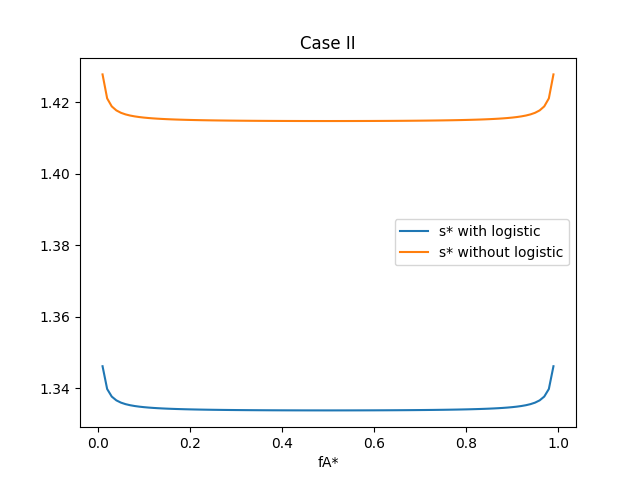
\includegraphics[width=4.5cm]{sstar_caseII}
	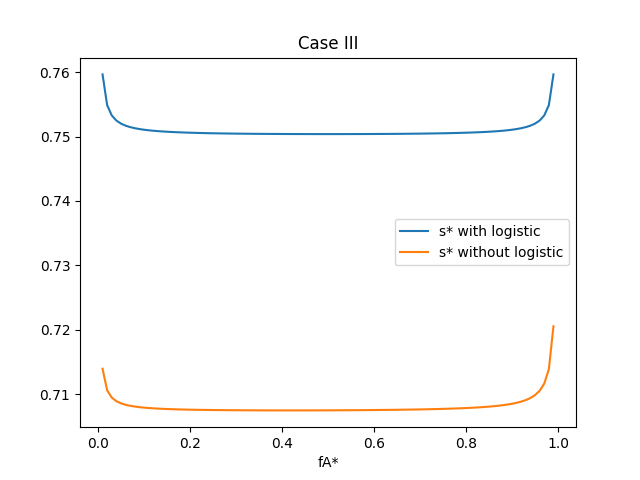
\includegraphics[width=4.5cm]{sstar_caseIII}
	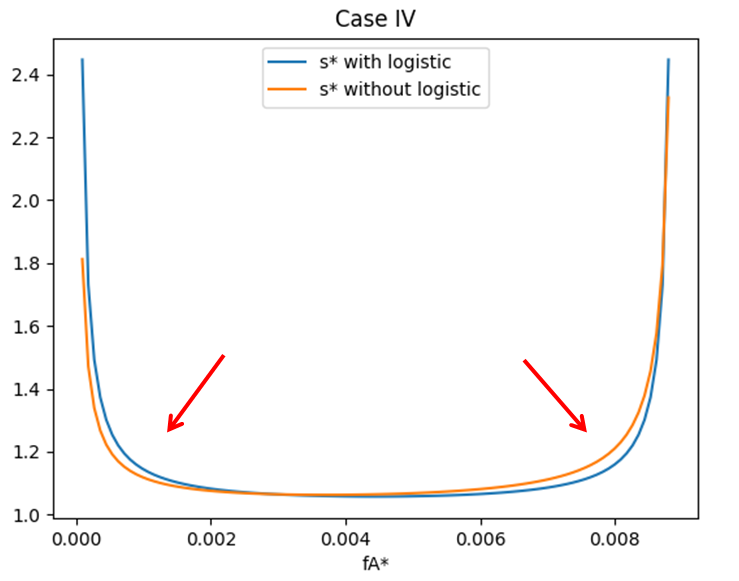
\includegraphics[width=4cm]{caseIVmodi}
	\caption{Placeholder critical values}
\end{figure}


\begin{itemize}
	\item case $s^{*}_{C}<s^*_{L}$. If $s< s^{*}_{c}$ we should observe stability for both model, if $s \in (s^{*}_C, s^{*}_L)$ we should observe instability for model and no aggregates for with logistic one. In the case of $s>s^{*}_{L}$ we expect instability and cell aggregates for both models. 
	\item case $s^{*}_{C}>s^*_{L}$. We should observe the opposite behavior compared to the previous one and instability for logistic model and no aggregates for the other one when  $s \in (s^{*}_L, s^{*}_C)$.
\end{itemize}


In the next section we will discuss some numerical simulations on the individual agent-based model to confirm the results provided by stability analysis.




%%---simulation values---
%	\begin{center}
%	\begin{tabular}{ l |c|c|c| r }
%	\hline
%		Test & $\nu_b^{A}$ & $\nu_b^{B}$ & $s^{*}_{L}$ & s \\ 
%		\hline
%		I &  $10^{-5}$ & $10^{-4} $ & 1.9 & $1.7$ \\ 
%		% II & $5 \cdot 10^{-5}$  & $10^{-4}$ & $1.56$ & $1.51$   \\
%		IIIa & $10^{-4}$  & $10^{-4}$ & $1.39$ & $1.43$ \\
%		IIIb & $10^{-4}$  & $10^{-4}$ & $1.39$ & $1$ \\
%		IIIc & $10^{-4}$  & $10^{-4}$ & $1.39$ & $2$ \\
%		% IV  & $10^{-4}$ & $5\cdot 10^{-5}$ & $1.25$ & $1.35$ \\
%		V & $10^{-4}$ & $10^{-5}$ & $1.09$ & $1.3$ \\
%		
%	\hline
%	\end{tabular}
%	\end{center}








	\section{Numerical scheme}
	\subsection{Macroscopic model}
	
The equations for the macroscopic model can be written as:

\begin{equation}
 \p_t f^{S}=\Linkop(f^S,f^T)+\Difop(f^S)+\Logop(f^S,f^T), \quad S\neq T\in\{A,B\}
\end{equation}
with
\begin{equation}
\Linkop(f^S,f^T)=  \nabla \cdot (f^S\nabla_x(\Phi^{SS}* f^S)) + \nabla \cdot (f^S \nabla_x \Phi^{ST}*f^T)
\end{equation}
\begin{equation}
\Difop(f^S)= D_S \Delta_x f^S
\end{equation}
\begin{equation}
\Logop(f^S,f^T)=\nu^{S}f^S\left( 1-\frac{f^S+f^T}{f^{*}} \right)
\end{equation}


\subsubsection{Spatial Discretization}


First we focus on the spatial discretization of the equations. A general semi-discrete finite-volume scheme can be written as follows:
\begin{equation}
\frac{d f^{S}_{j,k}}{dt}=\Linkop_{j,k}+\Difop_{j,k}+\Logop_{j,k}
\end{equation}
The discrtization of the terms $\Difop_{j,k}$ and $\Logop_{j,k}$ is straightforward and we will present only the details for the link operator $\Linkop_{j,k}$. As in \textbf{citation}, we set :
\begin{equation}
\Linkop_{j,k}= -\frac{F^{x}_{j+\frac{1}{2},k}-F^{x}_{j-\frac{1}{2},k}}{\Delta x}-\frac{F^{y}_{j,k+\frac{1}{2}}-F^{y}_{j,k-\frac{1}{2}}}{\Delta y},
\end{equation}
with
\begin{equation*}
 F^{x}_{j+\frac{1}{2},k}=u^{+}_{j+\frac{1}{2},k}f^{E}_{j,k}-
u^{-}_{j+\frac{1}{2},k}f^{W}_{j+1,k}, \quad F^{y}_{j,k+\frac{1}{2}}=u^{+}_{j,k+\frac{1}{2}}f^{N}_{j,k}-
u^{-}_{j,k+\frac{1}{2}}f^{S}_{j,k+1}
\end{equation*}
% $$F^{x}_{j-\frac{1}{2},k}=u^{+}_{j-\frac{1}{2},k}f^{E}_{j-1,k}-
% u^{-}_{j-\frac{1}{2},k}f^{W}_{j,k}, \quad F^{y}_{j,k-\frac{1}{2}}=u^{+}_{j,k-\frac{1}{2}}f^{N}_{j,k-1}-
% u^{-}_{j,k-\frac{1}{2}}f^{S}_{j,k}$$
where $u^{+}=\max(u,0)$, $u^{-}=-\min(u,0)$ and with 

$$u_{j+\frac{1}{2},k}=-\frac{\xi_{j+1,k}-\xi_{j,k}}{\Delta x}, \quad u_{j,k+\frac{1}{2}}=-\frac{\xi_{j,k+1}-\xi_{j,k}}{\Delta y}$$.

% $$u_{j-\frac{1}{2},k}=-\frac{\xi_{j,k}-\xi_{j-1,k}}{\Delta x}, \quad u_{j,k-\frac{1}{2}}=-\frac{\xi_{j,k}-\xi_{j,k-1}}{\Delta y}$$.

$$ \xi_{j,k}=\Delta x \Delta y \sum_{i,\l} \tilde{\Phi}^{SS}_{j-i,k-\l} f^{S}_{i,\l}+
\tilde{\Phi}^{ST}_{j-i,k-\l} f^{T}_{i,\l} $$
with ${\Phi}^{SS}(x_j-x_i,x_k-x_{\l})$. We compute te convolution term with a FFT method.
% $$ \xi_{j,k}=\Delta x \Delta y \sum_{i} \sum_{\l} \tilde{\Phi}^{AA}(x_{j}-x_{i},x_{k}-x_{\l}) f^{A}_{i,\l}+
% \tilde{\Phi}^{AB}(x_{j}-x_{i},x_{k}-x_{\l}) f^{B}_{i,\l} $$
% 
% $$ F_R=\nu_b^{A}f^{A}_{j,k}\left(1-\frac{f^{A}_{j,k}+f^{B}_{j,k}}{f^{*}}\right). $$


\subsubsection{Time Discretization}

The time discretization of the equations is done with an Euler scheme. The diffusion term is treated implicitly whereas the link term and the logistic term are treated explicitly. This leads to the following scheme:
\begin{equation}
	\frac{f_{j,k}^{S,n+1}-f_{j,k}^{S,n}}{\Delta t}=\Linkop_{j,k}^n+\Difop_{j,k}^{n+1}+\Logop_{j,k}^n
\end{equation}
%  $$(LO)^{n}=-\frac{F^{x,n}_{j+\frac{1}{2},k}-F^{x,n}_{j-\frac{1}{2},k}}{\Delta x}-\frac{F^{y,n}_{j,k+\frac{1}{2}}-F^{y,n}_{j,k-\frac{1}{2}}}{\Delta y}.	$$
\subsection{Microscopic model}
We perform numerical simulations on a $2D$ domain as in [cit] $[-L, L]\times[-L,L]=[-7.5,7.5]^2$ with periodic boundary conditions. We set diffusion constants $D_A=D_B=10^{-4}$ and investigate different values of inter- and intra- species intensities such as $\ka^{AA}, \ka^{BB}, \ka^{AB}=s\tilde{\ka}^{AB},  \ka^{BA}=s\tilde{\ka}^{BA}.$ For each equation of system \eqref{micro} we have the following time discretization:

\begin{equation}
X_i^{n+1}=X_i^{n}-\mu\nabla_{X_i} W(X^n)\Delta t^n+\sqrt{2D \Delta t^n}\mathcal{N}(0,1)
\end{equation}
 $\mathcal{N}(0,1)$ is the normal distribution with mean 0 and standard
deviation 1. \\
By the addition of logistic growth term in the model, the number of particles $N_A, N_B$ changes at each time step. Daughter cells are supposed to born at distance $r$ from 'parent' cells that divide themselves. In our model we set $r=0.5$.

%% R related to link term (repulsion)
%% R0 related to logistic term (distance for birth and death)
%% r related to distance between parents and daughter cells

% logistic term
\begin{equation}
\beta_{A}=b_{0}^{A}-(b_{0}^{A}-\theta_{A})\left(\frac{N_A+N_B}{N^{*}}\right), \quad\quad \delta_{A}=d_{0}^{A}+(\theta_{A}-d_{0}^{A})\left(\frac{N_A+N_B}{N^{*}}\right)
\end{equation}


\section{Results}

	\begin{center}
	\begin{tabular}{ l | c | r }
		\hline
		Parameters & Values $A, B$ & Description \\ \hline
		L & $7.5$ & Length half size demain  \\ 
		R & ? &  radius \\
	
		$\mu$ & 1  & ..\\
		$\nu_c$  & .&  . \\
		$\nu_d$  & .&  . \\
		k & . & .\\
		D & & \\
		$\beta$ & & \\
		$\delta$ & & \\
		%	$N_A$ & 250 & particles of type A\\
%	$N_B$ & 250 & particles of type B \\
		\hline
	\end{tabular}
\end{center}	




%----------PLOTS
% DO NOT DELETE - NE PAS EFFACHER ---------------------
%\begin{figure}
%	\centering
%	\begin{minipage}[h]{%0.5\linewidth}
%	\centering
%	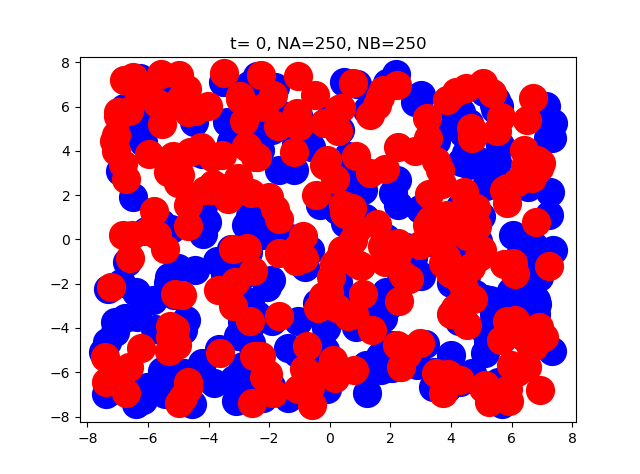
\includegraphics[width=1\linewidth]{micro_ini_caseI1}
%	%\captionof{figure}{ }\label{fig:1}
%	\end{minipage}
%\hfill
%	\begin{minipage}[h]{%0.5\linewidth}
%	\centering
%	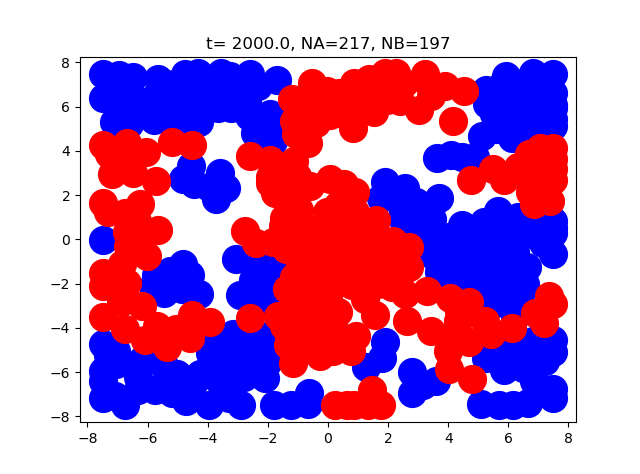
\includegraphics[width=1\linewidth]{micro_fin_caseI1}
%	%\captionof{figure}{ }\label{fig:2}
%	
%%{case I: A-cells blue, B-cells red with $k^{AA}=k^{BB}=2 $, $k^{AB}=k^{BA}=8$; $b0_A=b0_B=10^{-3}$, $d0_A=d0_B=7\cdot10^{-4}$}	
%	\end{minipage}
%\end{figure}
%-----------------------------------------------------

% DO NOT DELETE - NE PAS EFFACHER
%2: {case I: A-cells blue, B-cells red with $k^{AA}=k^{BB}=2 $, $k^{AB}=k^{BA}=8$; $b0_A=b0_B=2\cdot10^{-3}$, $d0_A=d0_B=7\cdot10^{-4}$}

%3: {case I: A-cells blue, B-cells red with $k^{AA}=k^{BB}=2 $, $k^{AB}=k^{BA}=8$; $b0_A=b0_B=10^{-4}$, $d0_A=d0_B=7\cdot10^{-5}, \th_A=\th_B=8\cdot 10^{-5}$}

%4: {case I: A-cells blue, B-cells red with $k^{AA}=k^{BB}=2 $, $k^{AB}=k^{BA}=4$; $b0_A=b0_B=10^{-4}$, $d0_A=d0_B=7\cdot10^{-5}, \th_A=\th_B=8\cdot 10^{-5}$}

%5: {case I: A-cells blue, B-cells red with $k^{AA}=k^{BB}=2 $, $k^{AB}=k^{BA}=2$; $b0_A=b0_B=10^{-4}$, $d0_A=d0_B=10^{-5}, \th_A=\th_B=8\cdot 10^{-5}$}

%6: {case I: A-cells blue, B-cells red with $k^{AA}=k^{BB}=2 $, $k^{AB}=k^{BA}=2$; $b0_A=b0_B=10^{-4}$, $d0_A=d0_B=10^{-5}, \th_A=\th_B=8\cdot 10^{-5}$}



\begin{figure}[htb]
	\begin{minipage}[t]{.45\textwidth}
		\centering
		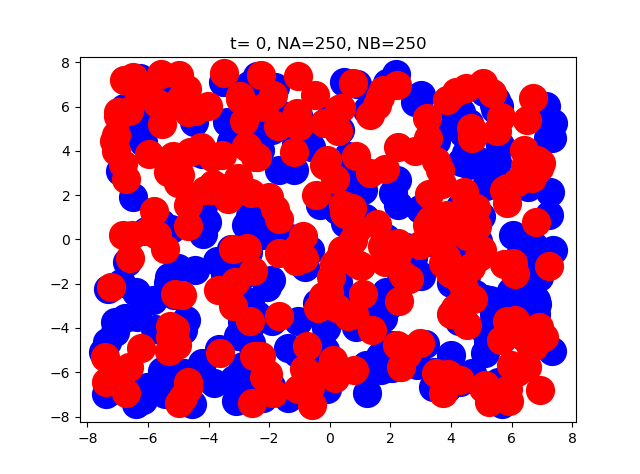
\includegraphics[width=\textwidth]{micro_ini_caseI1}
	%	\subcaption{Image 1.}\label{fig:1}
	\end{minipage}
	\hfill
	\begin{minipage}[t]{.45\textwidth}
		\centering
		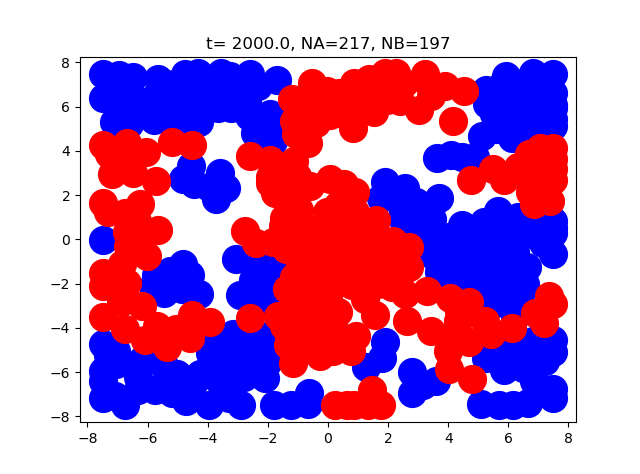
\includegraphics[width=\textwidth]{micro_fin_caseI1}
	%	\subcaption{Image 2.}\label{fig:2}
	\end{minipage}  
	\label{fig:1-2}
	\caption{{case I: A-cells blue, B-cells red with $k^{AA}=k^{BB}=2 $, $k^{AB}=k^{BA}=8$; $b0_A=b0_B=10^{-3}$, $d0_A=d0_B=7\cdot10^{-4}$}, $\th_A=\th_B=8\cdot 10^{-4}$}
\end{figure}


\begin{figure}[htb]
	\begin{minipage}[t]{.45\textwidth}
		\centering
		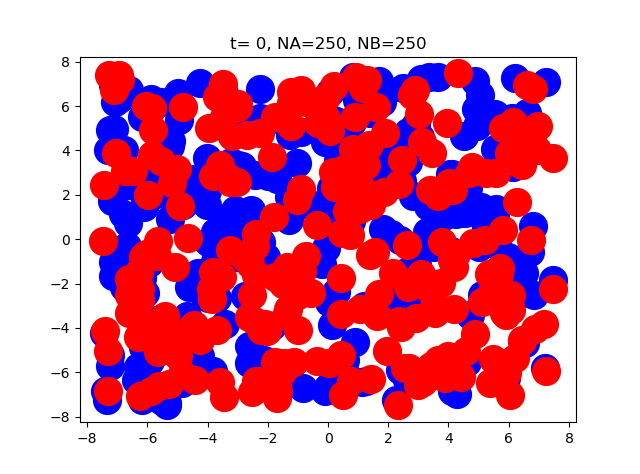
\includegraphics[width=\textwidth]{micro_caseI_ini2}
		%	\subcaption{Image 1.}\label{fig:1}
	\end{minipage}
	\hfill
	\begin{minipage}[t]{.45\textwidth}
		\centering
		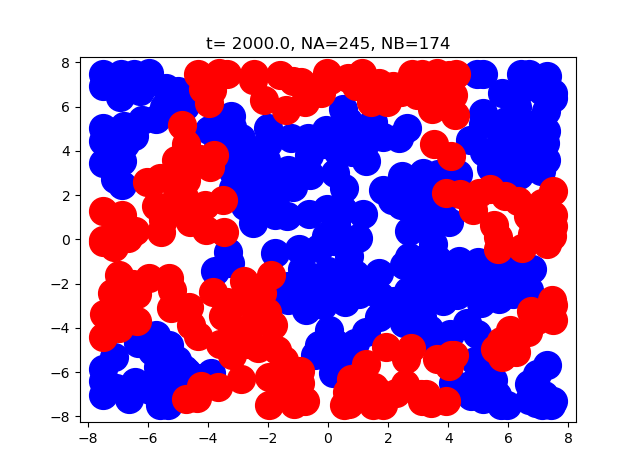
\includegraphics[width=\textwidth]{micro_caseI_fin2}
		%	\subcaption{Image 2.}\label{fig:2}
	\end{minipage}  
	\label{fig:1-2}
	\caption{{case I: A-cells blue, B-cells red with $k^{AA}=k^{BB}=2 $, $k^{AB}=k^{BA}=8$; $b0_A=b0_B=2\cdot10^{-3}$, $d0_A=d0_B=7\cdot10^{-4}$, $\th_A=\th_B=8\cdot 10^{-4}$}	}
\end{figure}


\begin{figure}[htb]
	\begin{minipage}[t]{.45\textwidth}
		\centering
		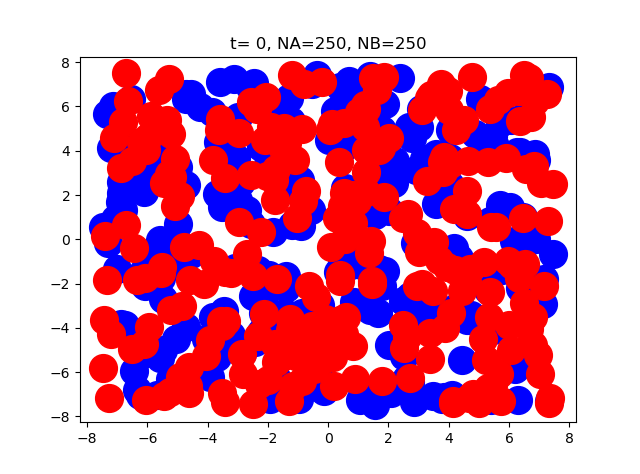
\includegraphics[width=\textwidth]{micro_caseI_ini3}
		%	\subcaption{Image 1.}\label{fig:1}
	\end{minipage}
	\hfill
	\begin{minipage}[t]{.45\textwidth}
		\centering
		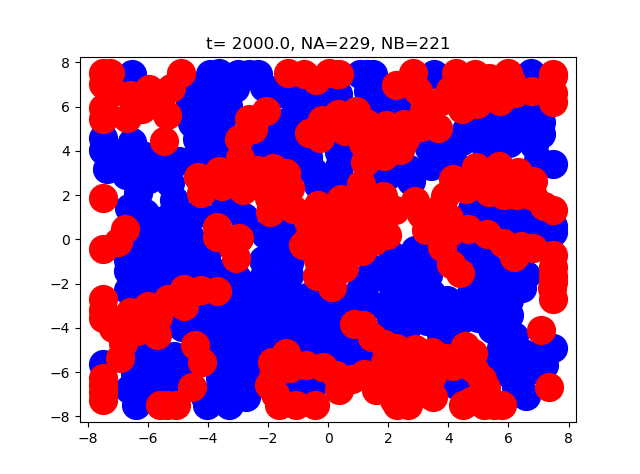
\includegraphics[width=\textwidth]{micro_caseI_fin3}
		%	\subcaption{Image 2.}\label{fig:2}
	\end{minipage}  
	\label{fig:1-2}
	\caption{{case I: A-cells blue, B-cells red with $k^{AA}=k^{BB}=2 $, $k^{AB}=k^{BA}=8$; $b0_A=b0_B=10^{-4}$, $d0_A=d0_B=7\cdot10^{-5}, \th_A=\th_B=8\cdot 10^{-5}$}	}
\end{figure}



\begin{figure}[htb]
	\begin{minipage}[t]{.45\textwidth}
		\centering
		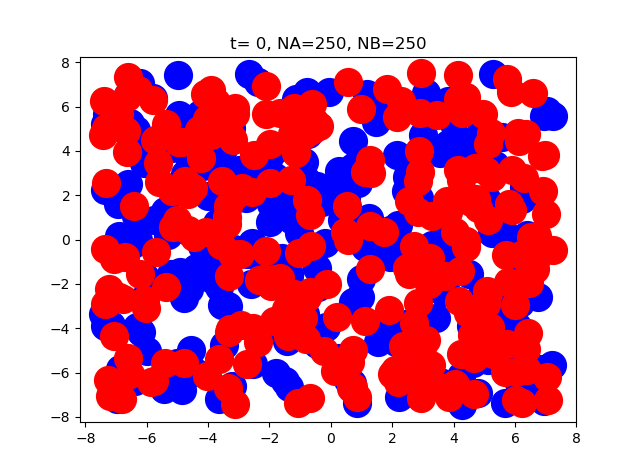
\includegraphics[width=\textwidth]{micro_caseI_ini4}
		%	\subcaption{Image 1.}\label{fig:1}
	\end{minipage}
	\hfill
	\begin{minipage}[t]{.45\textwidth}
		\centering
		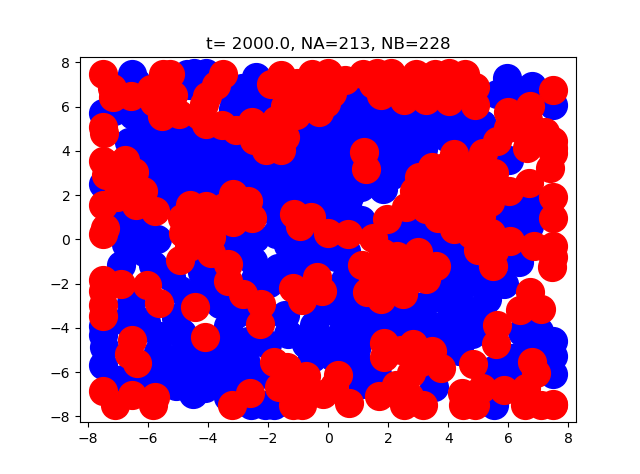
\includegraphics[width=\textwidth]{micro_caseI_fin4}
		%	\subcaption{Image 2.}\label{fig:2}
	\end{minipage}  
	\label{fig:1-2}
	\caption{{case I: A-cells blue, B-cells red with $k^{AA}=k^{BB}=2 $, $k^{AB}=k^{BA}=4$; $b0_A=b0_B=10^{-4}$, $d0_A=d0_B=7\cdot10^{-5}, \th_A=\th_B=8\cdot 10^{-5}$}	}
\end{figure}


\begin{figure}[htb]
	\begin{minipage}[t]{.45\textwidth}
		\centering
		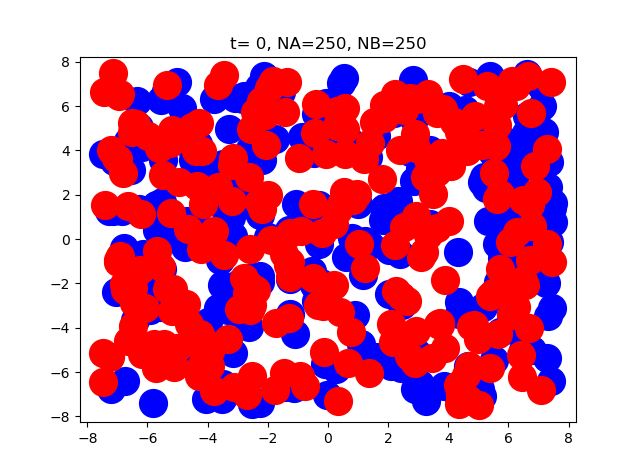
\includegraphics[width=\textwidth]{micro_caseI_ini5}
		%	\subcaption{Image 1.}\label{fig:1}
	\end{minipage}
	\hfill
	\begin{minipage}[t]{.45\textwidth}
		\centering
		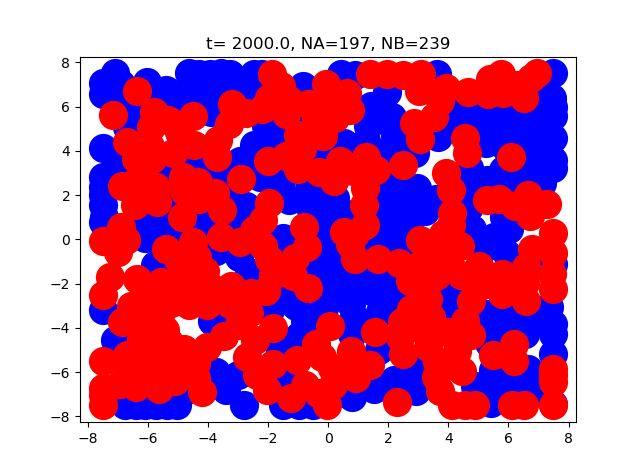
\includegraphics[width=\textwidth]{micro_caseI_fin5}
		%	\subcaption{Image 2.}\label{fig:2}
	\end{minipage}  
	\label{fig:1-2}
	\caption{{case I: A-cells blue, B-cells red with $k^{AA}=k^{BB}=2 $, $k^{AB}=k^{BA}=2$; $b0_A=b0_B=10^{-4}$, $d0_A=d0_B=10^{-5}, \th_A=\th_B=8\cdot 10^{-5}$}}
\end{figure}



\begin{figure}[htb]
	\begin{minipage}[t]{.45\textwidth}
		\centering
		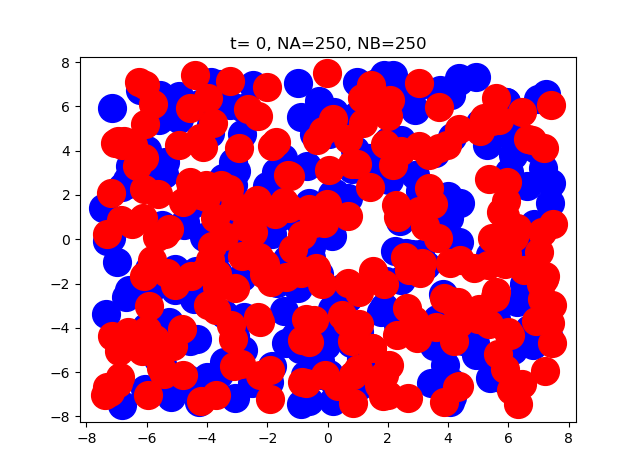
\includegraphics[width=\textwidth]{micro_caseII_ini1}
		%	\subcaption{Image 1.}\label{fig:1}
	\end{minipage}
	\hfill
	\begin{minipage}[t]{.45\textwidth}
		\centering
		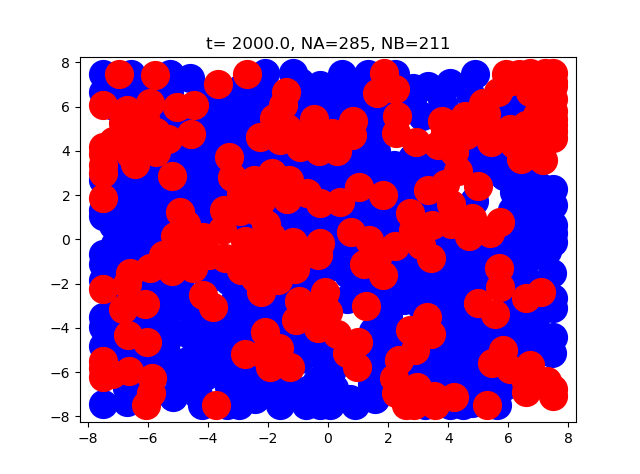
\includegraphics[width=\textwidth]{micro_caseII_fin1}
		%	\subcaption{Image 2.}\label{fig:2}
	\end{minipage}  
	\label{fig:1-2}
	\caption{{case II logistic: A-cells blue, B-cells red with $k^{AA}=k^{BB}=2 $, $k^{AB}=1.38, k^{BA}=2\cdot k^{AB}$; $b0_A=b0_B=10^{-4}$, $d0_A=d0_B=10^{-5}, \th_A=\th_B=8\cdot 10^{-5}$}}
\end{figure}


\begin{figure}[htb]
	\begin{minipage}[t]{.45\textwidth}
		\centering
		\includegraphics[width=\textwidth]{micro_caseII_ini2}
		%	\subcaption{Image 1.}\label{fig:1}
	\end{minipage}
	\hfill
	\begin{minipage}[t]{.45\textwidth}
		\centering
		\includegraphics[width=\textwidth]{micro_caseII_fin2}
		%	\subcaption{Image 2.}\label{fig:2}
	\end{minipage}  
	\label{fig:1-2}
	\caption{{case II NO logistic: A-cells blue, B-cells red with $k^{AA}=k^{BB}=2 $, $k^{AB}=1.38, k^{BA}=2\cdot k^{AB}$.}}
\end{figure}


\begin{figure}[htb]
	\begin{minipage}[t]{.45\textwidth}
		\centering
		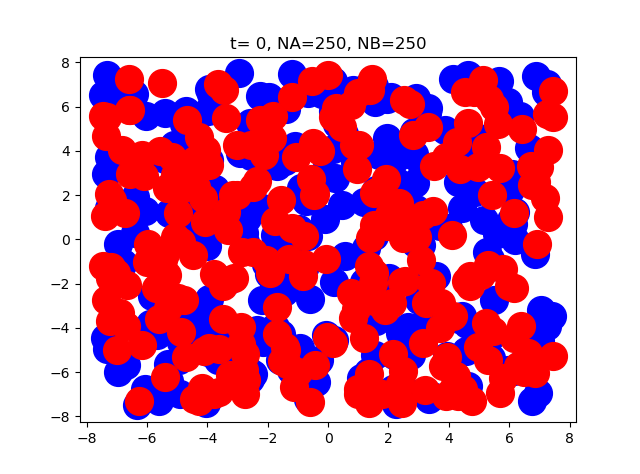
\includegraphics[width=\textwidth]{micro_caseIII_ini}
		%	\subcaption{Image 1.}\label{fig:1}
	\end{minipage}
	\hfill
	\begin{minipage}[t]{.45\textwidth}
		\centering
		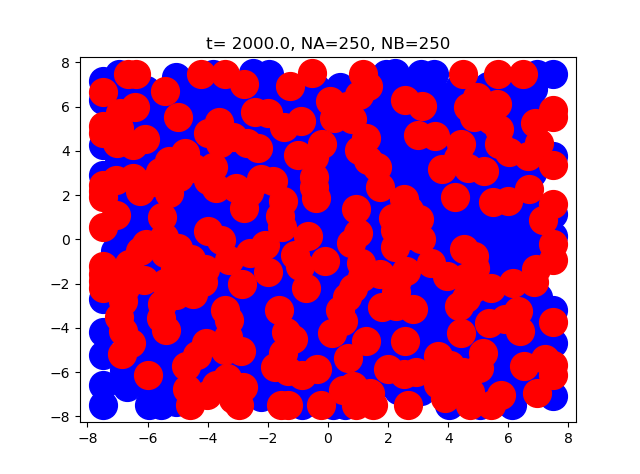
\includegraphics[width=\textwidth]{micro_caseIII_fin}
		%	\subcaption{Image 2.}\label{fig:2}
	\end{minipage}  
	\label{fig:1-2}
	\caption{{case III NO logistic ($s^{*}_{c} < s^{*}_{L}$): A-cells blue, B-cells red with $k^{AA}=2, k^{BB}=1 $, $k^{AB}=k^{BA}=2\cdot 0.73$.}}
% $s*_{c} circa 0.71 < s*_{L} circa 0.75 $
\end{figure}















%\section{Results}





\clearpage{\pagestyle{empty}\cleardoublepage}
%\lhead[\fancyplain{}{\bfseries\thepage}]{\fancyplain{}{\bfseries\rightmark}}
\begin{thebibliography}{20} 
	%	\pagenumbering{roman}
	%	\addcontentsline{toc}{chapter}{Bibliography} 
	\bibitem{}{J. Barré, P. Degond, E. Zatorska. Kinetic theory of particle interactions mediated by dynamical networks. SIAM MMS (2017) 15(3): 1294-1323.} 
	
	\bibitem{}{J. Barré, J.A. Carrillo, P. Degond, D.Peurichard, E. Zatorska. Particle interactions mediated by dynamical networks: assessment of macroscopic description. Nonlinear sci (2017). https://doi.org/10.1007/s00332-017-9408-z.} 
	\bibitem{}{J. Barré, J.A. Carrillo, P. Degond, D.Peurichard, E. Zatorska. A two-species macroscopic model for cell segregation and border sharpening by Eph receptor ephrin-mediated repulsion. \textit{In preparation}}
	\bibitem{}{J. A. Carrillo, A. Chertock, Y. Huang. A finite-volume method for Nonlinear Nonlocal Equations with a Gradient Flow Structure. Commun. Comput. Phys. (2015), 17(1):233-258.}
	% https://doi.org/10.4208/cicp.160214.010814a.
	
\end{thebibliography} 
	
\end{document}